%-----------------------------------------------------------------------------
%
%               Template for sigplanconf LaTeX Class
%
% Name:         sigplanconf-template.tex
%
% Purpose:      A template for sigplanconf.cls, which is a LaTeX 2e class
%               file for SIGPLAN conference proceedings.
%
% Guide:        Refer to "Author's Guide to the ACM SIGPLAN Class,"
%               sigplanconf-guide.pdf
%
% Author:       Paul C. Anagnostopoulos
%               Windfall Software
%               978 371-2316
%               paul@windfall.com
%
% Created:      15 February 2005
%
%-----------------------------------------------------------------------------

\documentclass[10pt]{sigplanconf}

% The following \documentclass options may be useful:

% preprint      Remove this option only once the paper is in final form.
% 10pt          To set in 10-point type instead of 9-point.
% 11pt          To set in 11-point type instead of 9-point.
% authoryear    To obtain author/year citation style instead of numeric.

\usepackage{amsmath}
\usepackage{epsfig}
\usepackage{alltt}
\usepackage{times}
\usepackage{array}
\usepackage{algorithm}
\usepackage{algorithmic}
\usepackage{graphicx}




%File mb-bibtex.tex, then \jobname = mb-bibtex
\RequirePackage{filecontents}        % loading package filecontents
% writing file \jobname.bib, for example mb-bibtex.bib.
\begin{filecontents*}{\jobname.bib}
@inproceedings{c1,
 author = {Stephenson, Mark and Amarasinghe, Saman},
 title = {Predicting Unroll Factors Using Supervised Classification},
 booktitle = {Proceedings of the International Symposium on Code Generation and Optimization},
 series = {CGO '05},
 year = {2005},
 isbn = {0-7695-2298-X},
 pages = {123--134},
 numpages = {12},
 url = {http://dx.doi.org/10.1109/CGO.2005.29},
 doi = {10.1109/CGO.2005.29},
 acmid = {1048981},
 publisher = {IEEE Computer Society},
 address = {Washington, DC, USA},
} 

@article{c2,
 author = {Cooper, Keith D. and Schielke, Philip J. and Subramanian, Devika},
 title = {Optimizing for Reduced Code Space Using Genetic Algorithms},
 journal = {SIGPLAN Not.},
 issue_date = {July 1999},
 volume = {34},
 number = {7},
 month = may,
 year = {1999},
 issn = {0362-1340},
 pages = {1--9},
 numpages = {9},
 url = {http://doi.acm.org/10.1145/315253.314414},
 doi = {10.1145/315253.314414},
 acmid = {314414},
 publisher = {ACM},
 address = {New York, NY, USA},
} 


@inproceedings{c3,
 author = {Monsifrot, Antoine and Bodin, Fran\c{c}ois and Quiniou, Rene},
 title = {A Machine Learning Approach to Automatic Production of Compiler Heuristics},
 booktitle = {Proceedings of the 10th International Conference on Artificial Intelligence: Methodology, Systems, and Applications},
 series = {AIMSA '02},
 year = {2002},
 isbn = {3-540-44127-1},
 pages = {41--50},
 numpages = {10},
 url = {http://dl.acm.org/citation.cfm?id=646053.677574},
 acmid = {677574},
 publisher = {Springer-Verlag},
 address = {London, UK, UK},
 keywords = {boosting, compiler heuristics, decision tree, loop unrolling},
}

@inproceedings{c4,
 author = {Cavazos, John and Moss, J. Eliot B.},
 title = {Inducing Heuristics to Decide Whether to Schedule},
 booktitle = {Proceedings of the ACM SIGPLAN 2004 Conference on Programming Language Design and Implementation},
 series = {PLDI '04},
 year = {2004},
 isbn = {1-58113-807-5},
 location = {Washington DC, USA},
 pages = {183--194},
 numpages = {12},
 url = {http://doi.acm.org/10.1145/996841.996864},
 doi = {10.1145/996841.996864},
 acmid = {996864},
 publisher = {ACM},
 address = {New York, NY, USA},
 keywords = {Java, Jikes RVM, compiler optimization, instruction scheduling, machine learning, supervised learning},
} 


@inproceedings{c5,
 author = {Agakov, F. and Bonilla, E. and Cavazos, J. and Franke, B. and Fursin, G. and O'Boyle, M. F. P. and Thomson, J. and Toussaint, M. and Williams, C. K. I.},
 title = {Using Machine Learning to Focus Iterative Optimization},
 booktitle = {Proceedings of the International Symposium on Code Generation and Optimization},
 series = {CGO '06},
 year = {2006},
 isbn = {0-7695-2499-0},
 pages = {295--305},
 numpages = {11},
 url = {http://dx.doi.org/10.1109/CGO.2006.37},
 doi = {10.1109/CGO.2006.37},
 acmid = {1122412},
 publisher = {IEEE Computer Society},
 address = {Washington, DC, USA},
} 

@article{c6,
 author = {Cavazos, John and O'Boyle, Michael F. P.},
 title = {Method-specific Dynamic Compilation Using Logistic Regression},
 journal = {SIGPLAN Not.},
 issue_date = {October 2006},
 volume = {41},
 number = {10},
 month = oct,
 year = {2006},
 issn = {0362-1340},
 pages = {229--240},
 numpages = {12},
 url = {http://doi.acm.org/10.1145/1167515.1167492},
 doi = {10.1145/1167515.1167492},
 acmid = {1167492},
 publisher = {ACM},
 address = {New York, NY, USA},
 keywords = {Java, Jikes RVM, compiler optimization, logistic regression, machine learning},
} 

@inproceedings{c7,
 author = {Cavazos, John and Fursin, Grigori and Agakov, Felix and Bonilla, Edwin and O'Boyle, Michael F. P. and Temam, Olivier},
 title = {Rapidly Selecting Good Compiler Optimizations Using Performance Counters},
 booktitle = {Proceedings of the International Symposium on Code Generation and Optimization},
 series = {CGO '07},
 year = {2007},
 isbn = {0-7695-2764-7},
 pages = {185--197},
 numpages = {13},
 url = {http://dx.doi.org/10.1109/CGO.2007.32},
 doi = {10.1109/CGO.2007.32},
 acmid = {1252540},
 publisher = {IEEE Computer Society},
 address = {Washington, DC, USA},
} 

@article{c8,
 author = {Cooper, Keith D. and Subramanian, Devika and Torczon, Linda},
 title = {Adaptive Optimizing Compilers for the 21st Century},
 journal = {J. Supercomput.},
 issue_date = {August 2002},
 volume = {23},
 number = {1},
 month = aug,
 year = {2002},
 issn = {0920-8542},
 pages = {7--22},
 numpages = {16},
 url = {http://dx.doi.org/10.1023/A:1015729001611},
 doi = {10.1023/A:1015729001611},
 acmid = {603341},
 publisher = {Kluwer Academic Publishers},
 address = {Hingham, MA, USA},
 keywords = {biased random search, configurable compilers, optimizing compilers, order of optimization},
}

@article{c9,
 author = {Cooper, Keith D. and Grosul, Alexander and Harvey, Timothy J. and Reeves, Steven and Subramanian, Devika and Torczon, Linda and Waterman, Todd},
 title = {ACME: Adaptive Compilation Made Efficient},
 journal = {SIGPLAN Not.},
 issue_date = {July 2005},
 volume = {40},
 number = {7},
 month = jun,
 year = {2005},
 issn = {0362-1340},
 pages = {69--77},
 numpages = {9},
 url = {http://doi.acm.org/10.1145/1070891.1065921},
 doi = {10.1145/1070891.1065921},
 acmid = {1065921},
 publisher = {ACM},
 address = {New York, NY, USA},
 keywords = {adaptive compilation},
} 


\end{filecontents*}


\usepackage[numbers]{natbib}         % bibliography style
\usepackage[colorlinks]{hyperref}    % better urls in bibliography



\newlength\myindent
\setlength\myindent{1em}
\newcommand\bindent{
  \begingroup
  \setlength{\itemindent}{\myindent}
  \addtolength{\algorithmicindent}{\myindent}
}
\newcommand\eindent{\endgroup}

\newlength\mysecindent
\setlength\mysecindent{2em}
\newcommand\quadindent{
  \begingroup
  \setlength{\itemindent}{\mysecindent}
  \addtolength{\algorithmicindent}{\mysecindent}
}
\newcommand\quadeindent{\endgroup}


\begin{document}

\special{papersize=8.5in,11in}
\setlength{\pdfpageheight}{\paperheight}
\setlength{\pdfpagewidth}{\paperwidth}


\doi{}

% Uncomment one of the following two, if you are not going for the 
% traditional copyright transfer agreement.

%\exclusivelicense                % ACM gets exclusive license to publish, 
                                  % you retain copyright

%\permissiontopublish             % ACM gets nonexclusive license to publish
                                  % (paid open-access papers, 
                                  % short abstracts)

%\titlebanner{banner above paper title}        % These are ignored unless
%\preprintfooter{short description of paper}   % 'preprint' option specified.

\title{Phase Ordering of Compiler Optimizations Using ML with Static and Dynamic Features}

\authorinfo{Ankit Goyal}
           {University of Texas at Austin}
           {ankit3goyal@gmail.com}

\authorinfo{Vivek Natarajan}
           {University of Texas at Austin}
           {natviv@gmail.com}



\maketitle

\begin{abstract}

Modern day compilers implement a number of optimizations. However, it is important to choose the right set of compiler optimizations and apply them in the right order as this can have a significant impact on program performance.  This is often referred to as the phase ordering problem of compiler optimizations in literature. However the optimizations interact in a complex manner with both the code and all other optimizations. Moreover the number of available optimization is also very high, hence the search space for the optimal optimization sequence is vast. Traditionally, compilers used pre-determined and generalized heuristics and apply the same set of optimizations in a fixed order regardless of the features of the program being optimized. In this project, we use an ensemble learning model based on a combination of performance counters, static code features and properties of the control flow graph learnt offline to predict a good set of compiler optimization sequences. We evaluate our learned model on a set of automatically generated programs using CSmith, a tool for generating random C programs that statically and dynamically conform to the C99 standard. Using our  method, we are able to demonstrate that a combination of static code features and performance counters performs better than the use of only static or performance counters for training the model. We obtain an average speedup of 17.32\% over the default order in the -O3 setting of the Clang compiler on our test set of automatically generated programs.   


\end{abstract}


\keywords
Machine Learning, Compilers, Hardware Counters, Optimizations

\section{Introduction}
The problem of determining the best set of optimizations for a particular program and their sequence, also known as the phase ordering, has been an open problem in compiler research. The problem is difficult because of two reasons. Firstly, modern day compiler implement a large number of optimization passes. For example, GCC has around 250 optimization passes and LLVM has at least 125 optimization passes implemented. However, because these optimizations transform the code in a non-linear manner, they could potentially alter the impact of other optimizations to be applied later. A classic example of this is the phase ordering problem between instruction scheduling and register allocation. Register allocation tries to make the optimum use of the available registers and prevent their spilling to the memory while instruction scheduling tries to reduce stalls by using more registers. This sort of phase ordering problem can arise between any pair of optimizations in a sequence. Hence it is imperative to select and schedule optimizations in a manner that their interactions are compatible and improve program performance. However, selecting the best sequence is highly non-trivial because the optimum solution may be located anywhere in this exponentially vast search space and the problem is thus NP-Hard.  

The standard practice in compilers is to use a fixed set of optimization passes (with a fixed sequence) corresponding to different levels of optimizations based on heuristics tuned on a fixed set of benchmark programs. Most of the optimization passes in GCC or LLVM are typically turned off and it is left to programmer to decide when and which set of optimizations to apply. However, it is obvious that the best set and ordering of optimizations varies from program to program. Traditional methods typically involve iterative compilation \cite{c1} or the use of genetic algorithms \cite{c2} to solve the phase ordering problem and efficiently scan the vast search space. Iterative compilation typically involves iteratively running  a set of optimizations on the program and using the performance to decide on a new optimization setting. Genetic algorithms were used by Cooper et al. \cite{c2} but involved the added constraint of optimizing for code size. Although they were able to reduce code size by as much as 40\%, the main bottleneck is they had to train the genetic algorithm for every program. These pure search techniques do use any apriori knowledge of the target machine, compiler or code under optimization instead iteratively evaluate and tune the heuristics to identify the best optimization setting. Cavazos et al. \cite{c7} suggest that this could take up to 600 evaluations of the program to zone in on the right optimization settings. In this project, we use a combination of performance counters, static code features and features of the control flow graph to learn a model offline and use it to predict the best optimization setting for the program under consideration. The performance counters are obtained from only three runs of a set of training programs. To the best of our knowledge, we are the first to use features of the control flow graph as static code features and also the first to use a combination of static code features and performance counters to tackle the phase ordering problem. Our results demonstrate that using the combination provides a significant improvement than using only one of static code features or performance counters as has been done in previous research.          

In recent times, Machine learning has received a lot of attention in problems pertaining to the selection of optimizations \cite{c4}  or even in cases like selection of the loop unroll factor \cite{c3}. Static code features were used by Agakov et al. \cite{c6} to identify a set of good optimizations to a program under test with the underlying assumption that optimizations which perform well on programs with similar static characteristics would perform well on the new program. However, static code features fail to model global characteristics of a program and fail when applied to large application programs especially those that are control-flow intensive. Cavazos et al. \cite{c7} came up with a solution  to this issue by using performance counters which have been extensively used in performance analysis of programs. However, they do not address the issue of combining static and performance counters as features to train the model. In our opinion, the two provide orthogonal characterizations of the program and should complement each other well and our results substantiate our intuition. Moreover, our use of features which explicitly characterize the control flow graph of the program under consideration in combination with the static code features gives performance on par with the use of performance counters. This suggests that the features characterizing the control flow graph could be used as a useful substitute for the performance counters especially in the context of a static compiler. 

\section{Motivation}

Previous work by Agakov et al. \cite{c5} have demonstrated the use of static program features to characterize a program. Moreover the authors used a set of 36 features and demonstrated by using a Principal Component Analysis technique that the 99\% of the variance captured by this set could be captured by using a smaller subset of 5 features. Hence, for our experiments we chose a set of 9 program features which we felt best characterized our programs and could have a maximum impact on the optimization passes considered. The use of performance counters is motivated by Cavazos et al.\cite{7} demonstrated that performance counters could prove effective as features. However, the problem they solve is not the phase ordering problem. They only attempt to predict what optimization passes should be enabled for any program based on a given subset. We also analyzed the control flow graph of the program to extract features corresponding to its shape for every function because a number of program optimizations indirectly depend on the shape of the Control flow graph like dominance relationships. \\


\section{Methodology}
\noindent
In this section, we describe our methodology for selecting the optimization passes considered for the phase ordering problem, the features used to characterize the program, construction of the training set and the learning model to predict the best optimization sequences for a new test program.


\subsection{Selection of the Optimization passes considered for the phase ordering problem:}
We considered the optimization passes listed in Table 1, (available in LLVM) for the phase ordering optimization. Most of the previous research do not really explain their reasons for  selecting the optimization passes. In this project, we chose a set of passes which could potentially have a significant impact on the static code features and performance counters. Passes like function inline and reassociate have a strong correlation with the CFG and static code features. On the other hand optimizations like loop invariant code motion and  loop-unroll have a direct impact on cache utilization and/or in the number of memory operations. It should be noted that majority of passes impact both static and dynamic features. As demonstrated previously, the ordering of the passes does have a significant impact on the performance of the program.


\begin{table}[tbl1]
\caption{Set of optimizations used for phase order optimizations with their description}
\begin{tabular} {lll}
\hline
\bf{ LLVM Pass Name} & \bf{Pass Description} \\ \hline
-dse & Dead Store Elimination \\ \hline
-loop-unroll & Unroll Loops \\ \hline
-loop-unswitch & Unswitch loops \\ \hline
-licm & Loop Invariant Code Motion \\ \hline
-memcpyopt & MemCpy Optimization \\ \hline
-loop-rotate & Rotate Loops \\ \hline
-inline & Function Integration/Inlining \\ \hline
-reassociate & Reassociate Expressions \\ \hline
-sccp & Sparse Cond. Constant Propagation \\ \hline

\end{tabular}
\label{tb:tbl1}
\end{table}


\subsection{Feature selection}
Feature selection has been an important topic of research in Machine learning and several heuristics have been proposed. The most important criteria is to select features that best characterize the variance in the data under consideration and are sufficiently discriminative to learn a good learning model. Previous work on this problem have either used static code features (Agakov et al. \cite{c5} ) or performance counters (Cavazos et al.  \cite{c7}) . In this project, we consider the combination of  both static code features and performance counters for each program.


\subsubsection{Static Features}
Since a good number of our optimization passes deal with loops,  we have selected on program features related to loops in the code. We have a taken a subset of features used by Stephenson et al \cite{c1} as shown in Table 2. As stated previously, a small set of static features is often sufficient to capture the variance in the set of programs under consideration and we decided to focus on the small set of features listed in Table 2.  An LLVM pass to compute these features and we used the existing loop analysis pass provided by LLVM for some of the features. The features computed were averaged out if they were local in nature (“like pertaining to individual loops”) and normalize it by the number of instructions in the program for consistency among different programs. 


\subsubsection{Features obtained from the Control Flow Graph}

We used the LLVM -dot-cfg pass to obtain the graphs representing the Control Flow Graph (CFG) corresponding to each program in the program under consideration. We used the NetworkX and PyGraphViz library implemented in python to analyze the CFG for every function in the program under consideration and obtained features corresponding to the number of nodes, number of nodes, the average degree, the diameter, the clustering co-efficient, the average path length and the graph density - features which we believe effectively characterize the shape of the CFG. We aggregate these values for the CFG corresponding to each function in the program and take the average value as features in addition to the static features mentioned previously.    


\begin{table}[tbl2]
\caption{Static features used (subset of features used in \cite{c8})}
\begin{tabular} {lll}
\hline

\bf{Acronym} & \bf{Description} \\ \hline 
LoopInstNum & Num. of instructions in a loop \\ \hline 
LoopNum & Num. of loops \\ \hline 
LoopBasicBlocksNum & Num. of basic blocks in a loop \\ \hline 
LoopDepth & Average loop depth \\ \hline 
LoopBranchInstNum & Num. of branching instructions \\ \hline 
LoopLoadInst & Num. of Load instructions \\ \hline 
LoopStoreInst  & Num. of store instructions \\ \hline 
LoopNumOperands & Num. of operands in loop \\ \hline 
LoopNumMemInst & Num. of memory inst. in loop \\ \hline 
LoopNumOperations & Num. of operations in loop \\ \hline 

\end{tabular}
\label{tb:tbl2}
\end{table}



\begin{table*}[tbl3]
  \centering
  \begin{tabular}{l|l}

\hline

\bf{Performance Counter Name} & \bf{Performance Counter Meaning} \\ \hline
TOT\_INS & Total Number of Instructions \\ \hline
TOT\_CYC & Total Cycles \\ \hline
STL\_ICY & Cycles with no instruction issue \\ \hline
FP\_INS, FP\_OPS & Floating point instructions, operations \\ \hline
BR\_INS, BR\_MSP, BR\_TKN & Branch Instruction, Cond. Branches Mispredicted, Cond. Branches Taken \\ \hline
DCM, DCA, DCR, DCH, DCW & L1, L2 Data Cache: Accesses, Misses, Reads, Hits, Writes \\ \hline
LDM, STM & L1, L2 Cache: Load Misses, Store Misses \\ \hline
TCM, TCA & L1, L2 Total Cache Misses, Accesses \\ \hline
ICM, ICA & Instruction Cache: Misses, Accesses \\ \hline
TLB\_DM & Data translation lookup buffer misses \\ \hline
TLB\_IM & Instruction translation lookup buffer misses \\ \hline


  \end{tabular}
  \caption{Performance counters used as features. The performance counter name is the acronym used for the counters by PAPI library}
  \label{tab:tbl3}
\end{table*}

\subsubsection{Performance Counters}
To measure performance counters, most processors today have a special set of registers that can do this without any side effects on the execution of the program. These counters typically describe dynamic program characteristics like cache hits, misses and branch prediction accuracies. Performance counters were obtained using PAPI Hardware Counters library API. These counters are hardware specific and support for all the counters is not necessarily available on all the hardwares. We used the Stampede machine on TACC (2/8 Xeon E5-2680 2.7GHz) for all our experiments. A total of 25 performance counters were available on stampede based on the hardware and counter types; 8-10 hardware counters can be calculated in a single run. So we had to run each program 3 times to get all 25 counters. All the performance counters obtained were normalized by the total number of instructions in the program in order to allow for generalization regardless of the length of the program. The goal is to use the statistics obtained from static program features and dynamic performance as features to learn a good model for automatically predicting a good sequence of optimizations. 



\subsection{ Generation of the set of best optimization sequences}
In order to generate the training data, we considered all permutation of the optimization passes mentioned previously and obtained the execution times for our set of 27 different automatically generated programs. To do this efficiently, we divided the permutation into 4 and used OpenMP to parallelize the process of getting the execution times. All the programs were run on Stampede. We then sort the optimization sequences to obtain a set of 100 best optimization sequences and probabilistically compute a set of 5 best optimization sequences corresponding to each program.  


\subsection{ Ensemble Classifier }
We used the Exemplar SVM and Random Forest classifier as an ensemble classifier to predict a subset of optimization sequences for each program under test. Exemplar SVMs is a recently developed remodel of the conventional SVM classifier primarily tuned for meta-data transfer. It can be thought of as a combination of a discriminative and distance metric based Nearest Neighbor like classifier. The model is obtained by training a one vs all Linear SVM classifier for each positive instance in the training set consider vs a large set of negatives. In our case, our set of negatives is all the features corresponding to all the other programs bar the features corresponding to the program for which the model is being trained. Thus we train N different SVM classifiers and use the the predicted output of the classifier with the highest confidence. We also a train a separate random forest classifier and use it in an ensemble with the Exemplar SVM to obtain a prediction of the best optimization sequence for the program under test. We do a leave one out cross validation on all programs in training set and report our results. The classifiers were implemented using the scikit learn package in Python.



\section{Results}
We trained the classifier using three different kinds of features: first - we considered both static and dynamic features. Second - we consider only static features. Third - we consider only dynamic features. As can be seen in table 4. that we received a significant speedup in all three cases however speedup achieved is much greater in static + dynamic case than either the only static or only dynamic case.


\begin{table}[tbl4]
\caption{Speedup achieved in different cases.}
\begin{tabular} {|p{12em}|p{9em}|}
\hline

\bf{Method} & \bf{Avg. Speedup} \\ \hline
Static + CFG + Dynamic & 1.173250279 \\ \hline
Static + CFG & 1.107801959 \\ \hline
Dynamic & 1.102995532 \\ \hline

\end{tabular}
\label{tb:tbl4}
\end{table}


\subsection {Dynamic Features}
In this case only dynamic features are considered. Figure 1 shows average percentage improvement in execution time after applying the optimization passes in the predicted order over the default order of optimizations. It can be seen that in some cases the improvement is as high as 24\%. Average improvement in execution time over all programs is about 9.07\% which is very close to the 10\% speedup reported by Cavazos et al. \cite{c7} albeit on different benchmark programs.


\begin{figure}[ht!]
\centering
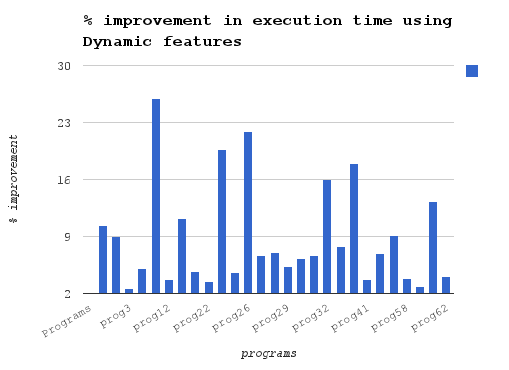
\includegraphics[width=80mm]{dynamic_exec_time.png}
\caption{Improvement in execution time using dynamic features}
\label{overflow}
\end{figure}


\subsection {Static Features}
In this case we only consider static features including CFG features. Figure 2. shows that in this case also we received a significant improvement in the execution time (as high as 27\%) of predicted order of optimization over the default order which is consistent with the results from paper Agakov et al.\cite{c5} Average improvement in execution time received in this case is 9.24\%

\begin{figure}[ht!]
\centering
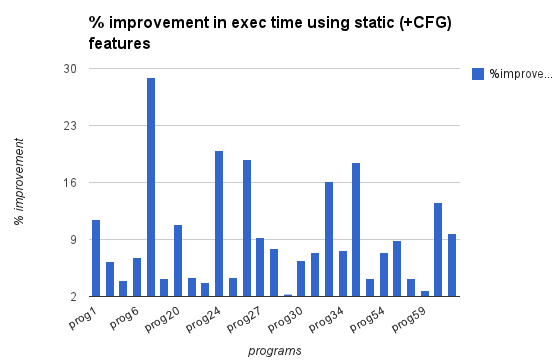
\includegraphics[width=80mm]{static_features.png}
\caption{Improvement in execution time using static features}
\label{overflow}
\end{figure}


\subsection {Dynamic and Static Features}
 According to the best of our knowledge our work is the first to consider both static program features and performance counters to characterize programs. As shown in Fig. 3 we were able to achieve much higher (upto 46\%) in some cases or at least the same amount of speedup in almost all cases. This results shows that some combination of both static and dynamic features will result in close to optimal performance.


\begin{figure}[ht!]
\centering
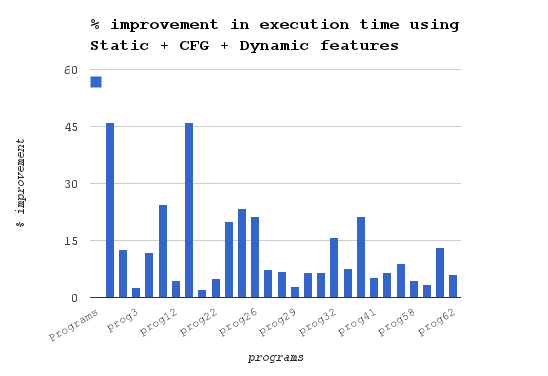
\includegraphics[width=80mm]{dyn_stat_features.png}
\caption{Improvement in execution time using static and dynamic features}
\label{overflow}
\end{figure}

\begin{figure}[ht!]
\centering
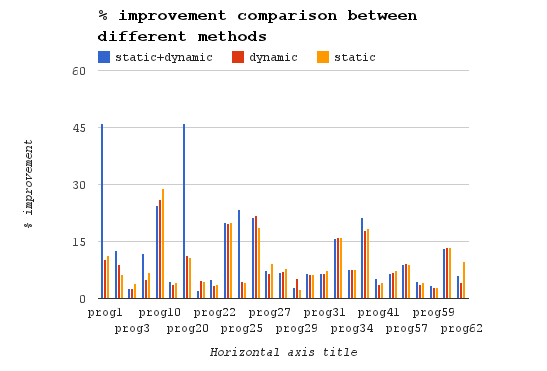
\includegraphics[width=80mm]{combined.png}
\caption{Comparison between improvement using different methods}
\label{overflow}
\end{figure}


\subsection {Impact of static features on phase order prediction}
The effect of same optimizations in different order can be seen in Figure 5 where predicted order has reduced the number of operations, memory instructions in the given program which directly impacts the execution time of the program.


We also observe variations in the CFG features obtained after applying the default order of optimizations and our predicted order. However, the variations are something which is consistent with our intuitions regarding compiler optimizations. However, their use is justified in the fact by the performance improvements obtained by the use of CFG features in addition to the traditional static features and performance counters.   

\begin{figure}[ht!]
\centering
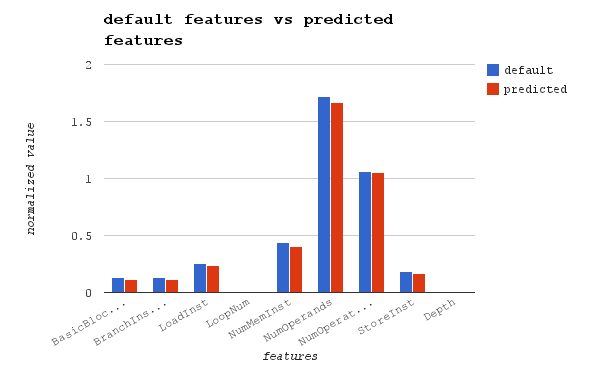
\includegraphics[width=80mm]{default_pred.png}
\caption{ Default phase order static features vs predicted phase order static features}
\label{overflow}
\end{figure}


\subsection { Impact of dynamic features on phase order prediction }

Figure 6. shows that our predicted order was able to improve cache utilization over the default optimization order used in -O3 flag of Clang for a program (prog20) in which we saw improvement of 46.09\%. Level 1 store misses reduced by 12.4\% while Level 2 data misses reduced by 10.3\%. It also reduced the TLB cache data misses by 21\%. It did worse on some other performance counters related to the the cache like TLB instruction misses increased by 16\%. However, we could generalize that it improved the cache performance over the default phase order. 

It is evident from the results that both static features and dynamic features are crucial in predicting the performance. Since we need to train our model just once, use of dynamic features is practical. All that is required is to execute the training programs on a new target machine to learn the model and using the model we can predict suitable optimization order for other unseen test programs without any sort of iterative execution. 




\begin{figure}[ht!]
\centering
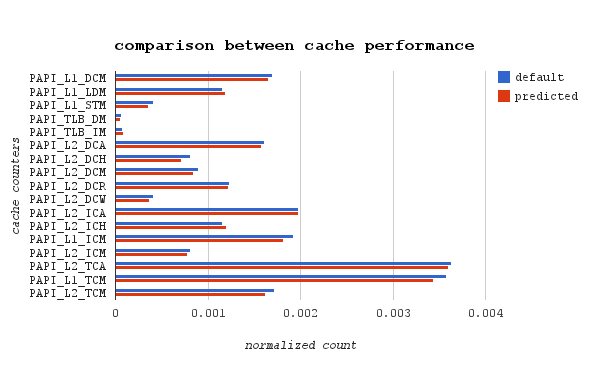
\includegraphics[width=80mm]{cache.png}
\caption{Cache performance of default order vs predicted order}
\label{overflow}
\end{figure}


\section{Related Work}

The phase ordering problem has been a open research topic in the field of Compilers for many years now. Traditional methods to tackle this problem have involved the use of iterative compilation \cite{c9} . Iterative compilation has been able to outperform the highest optimization settings in many compilers and also compares favourably when applied to many hand optimized vendor libraries. However, the key issue is it involves searching a combinatorially large space which could often take days or weeks to tune. Cooper et al. \cite{c9}  introduced a system called ACME to speedup iterative compilation using a technique called Virtual Execution which introduced a pass to analyze the CFG and identify advantages and disadvantages of applying specific optimizations. The technique works well on simple models but fails to estimate performance of out of order issue processors and requires changes to be made to each optimization pass of a compiler. 

Cooper et al. \cite{c8}  have also used genetic algorithms to solve the phase ordering problem. However, they were primarily concerned with selecting a sequence optimization for code size. Moreover, they had to retrain the model every time to optimize for a new program. 

The use of machine learning to construct heuristics to select near optimal phase orders has received considerable attention in recent years [\cite{c2},\cite{c3},\cite{c5}, \cite{c6},\cite{c7}]. Cavazos et al. \cite{c9}  used supervised learning techniques to decide whether instruction scheduling should be applied to basic blocks or not. Monsifrot et al. \cite{c3}  used a decision tree based classifier to determine which loops to unroll. Stephenson et al. [5] used genetic algorithms to tune heuristics for three compiler optimizations namely hyper block selection, data prefetching and register allocation. However, the key issue with all these works is they focus their attention on individual compiler optimizations, the heuristics perform poorly when considered in a sequence of compiler optimization. 

The work most similar to ours is the use of performance counters for optimization pass selection by Cavazos et al. \cite{c7}. However, it is important to note that it is not the phase ordering problem that they consider. Moreover, they only consider using performance counters while we have considered a combination of both static code features and dynamic performance counters and demonstrated significant speedup on our test set of automatically generated programs. 

\section{Conclusion and Future Work}
In this paper we address the phase ordering of compiler optimizations using machine learning techniques. To the best of our knowledge we are the first to consider both static code features and dynamic features in the performance counters. We saw significant improvement in the execution time (17.32\% avg.) by using both static and dynamic features. 

In the future we would like to test our method on several standard benchmarks and analyse if we get similar improvements in the execution times. Moreover we would also like to explore other optimization passes and their different combinations like allowing passes to occur multiple times or passes to not occur at all. It would also be interesting to include more complex features based on CFG. From our initial analysis static features including CFG features gave better results than  the use of traditional static features alone. We would like to develop a more principled approach to characterize the CFG and learn the model for predicting phase orders. 

We would also like to characterize the phase ordering problem as a sequence tagging problem like Markov Random Field or a Conditional Random Field often used in applications in NLP and Vision. We feel the phase ordering problem is amenable to such a formulation.





\bibliographystyle{plainnat}  % needs package natbib
\bibliography{\jobname}       % uses \jobname.bib, according to \jobname.tex



% We recommend abbrvnat bibliography style.
%\bibliographystyle{unsrt}

\acks
We would like to take this opportunity to thank Prof. Calvin Lin for the compilers course and motivating us for the project. We would also like to thank Arthur Peters for his suggestions.


\end{document}